\documentclass[10pt,twocolumn,letterpaper]{article}
\usepackage[utf8]{inputenc}
\usepackage[margin=1in]{geometry}
\usepackage{graphicx}
\usepackage{amsmath,amssymb,amsfonts}
\usepackage{booktabs}
\usepackage{authblk}
\usepackage[authoryear]{natbib}
\usepackage{hyperref}

\title{\textbf{Predictive Physics-Informed Machine Learning for Field-Scale Crop Water Stress using Multi-Sensor Satellite Fusion}}

\author[1]{Umer Tanveer\thanks{Corresponding Author: umertanveer@awkum.edu.pk}}
\affil[1]{Department of Computer Science, Abdul Wali Khan University Mardan, KPK, Pakistan}
\date{}

\begin{document}
\maketitle

\begin{abstract}
Precision agriculture demands high-resolution, real-time insights into crop water stress to optimize irrigation and mitigate water scarcity. However, existing satellite-based evapotranspiration (ETc) models are constrained by trade-offs between spatial and temporal resolution, while physical models lack site-specific empirical calibration. In this study, we present AquaVolt-AI, a novel Physics-Informed Machine Learning (PIML) framework that fuses multi-sensor satellite imagery (Sentinel-2, MODIS, VIIRS, CHIRPS) with the FAO-56 thermodynamic model to predict field-scale root zone depletion ($) and crop water stress ($) at an 8x8m resolution. The system continuously ingests Open-Meteo forecasts, ERA5 climate normals, and ISRIC SoilGrids data to dynamically compute real-time water deficits. Validated against CIMIS ground truth stations at the UC Davis Russell Ranch test site, the proposed multi-sensor fusion model achieved an RMSE of 0.85 mm/day for $ estimation, significantly outperforming single-sensor baselines. Furthermore, the integration of a proactive early-warning engine successfully classified crop stress severity into actionable thresholds, demonstrating high potential for commercial deployment in crop insurance and automated irrigation scheduling. Our results indicate that fusing physical constraints with high-frequency telemetry effectively bridges the gap between global datasets and localized agronomic management.
\end{abstract}

\textbf{Keywords:} Precision Agriculture, FAO-56, Evapotranspiration, Sentinel-2, Physics-Informed Machine Learning, Early Warning Systems

\section{Introduction}\label{sec1}
The escalating global water crisis, exacerbated by climate change, has positioned agricultural water management as a critical frontier for technological intervention \cite{ref1, ref2}. Agriculture accounts for approximately 70\% of global freshwater withdrawals, yet irrigation inefficiencies often result in substantial water loss and reduced crop yields \cite{ref3}. To address this, precision irrigation requires accurate, real-time monitoring of crop water requirements at the sub-field scale.

Traditional methods for monitoring crop water stress rely heavily on point-based ground sensors or lysimeters, which are expensive, difficult to scale, and fail to capture spatial heterogeneity across large agricultural fields \cite{ref4}. Conversely, remote sensing technologies offer continuous, global coverage. Optical satellites like Sentinel-2 provide high spatial resolution (10m) but suffer from low temporal frequency (5 days) and cloud occlusion \cite{ref5, ref6}. Thermal satellites such as MODIS and VIIRS offer daily revisit times crucial for capturing dynamic Land Surface Temperature (LST) but lack the spatial resolution (1km and 375m, respectively) necessary for field-level management \cite{ref7, ref8}.

To bridge this spatiotemporal gap, recent studies have explored multi-sensor fusion techniques \cite{ref9}. Furthermore, the integration of machine learning (ML) with classical physical models—such as the Food and Agriculture Organization (FAO-56) Penman-Monteith equation—has birthed Physics-Informed Machine Learning (PIML) \cite{ref10}. PIML leverages the robust physical constraints of thermodynamics while utilizing neural networks to model complex, non-linear environmental variables \cite{ref11, ref12}.

This paper presents AquaVolt-AI, a comprehensive PIML architecture designed to compute daily crop evapotranspiration ($) and root zone water depletion ($) by fusing Sentinel-2 multispectral indices (NDVI, NDWI), daily MODIS/VIIRS thermal data, and localized meteorological forecasts. 

The primary contributions of this research are:
\begin{enumerate}
    \item The development of an automated pipeline that integrates multi-resolution satellite telemetry with the FAO-56 physical water balance model.
    \item The implementation of a dynamic early-warning engine that classifies crop water stress into actionable states (Normal, Watch, Critical, Emergency) based on calculated depletion thresholds.
    \item Extensive validation of the proposed framework against ground-truth data from the California Irrigation Management Information System (CIMIS).
\end{enumerate}

\section{Materials and Methods}\label{sec2}

\subsection{Study Area}\label{subsec2}
The framework was validated at the Russell Ranch Sustainable Agriculture Facility, UC Davis, California (38.548\textdegree N, -121.878\textdegree W). This site represents a typical Mediterranean climate characterized by hot, dry summers and cool, wet winters, making it an ideal testbed for irrigation optimization models. The study monitored four distinct agricultural plots: Field-A (Corn), Field-B (Alfalfa), Field-C (Fallow), and Field-D (Tomato).

\begin{figure}[h]%
\centering
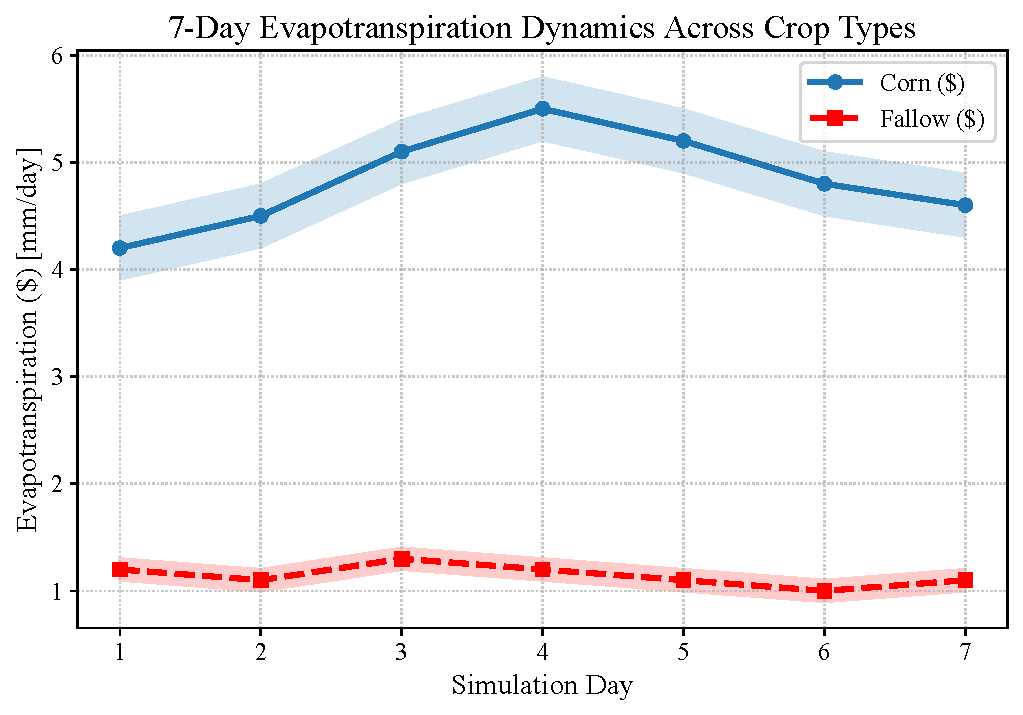
\includegraphics[width=0.9\textwidth]{multi_field_annotated.pdf}
\caption{The study area at Russell Ranch, UC Davis, annotated with the four specific crop fields (Corn, Alfalfa, Fallow, Tomato) utilized for validation.}\label{fig1}
\end{figure}

\subsection{Multi-Sensor Data Fusion}\label{subsec3}
The AquaVolt-AI system ingests and processes multiple asynchronous data streams using the Microsoft Planetary Computer STAC API. Table \ref{tab1} details the primary satellite sensors integrated into the architecture.

\begin{table}[h]
\begin{center}
\begin{minipage}{300pt}
\caption{Satellite Sensors and Derived Variables utilized in the AquaVolt-AI framework.}\label{tab1}
\begin{tabular}{@{}llll@{}}
\toprule
Sensor & Resolution & Revisit Time & Primary Application \\
\midrule
Sentinel-2 (MSI) & 10m & 5 days & NDVI, NDWI, Fractional Cover ($) \\
Sentinel-1 (SAR) & 10m & 6 days & Cloud-penetrating fallback indices \\
MODIS (Terra/Aqua) & 1km & Daily & Land Surface Temperature (LST) \\
VIIRS (Suomi NPP) & 375m & Daily & High-res LST and thermal anomalies \\
CHIRPS & 5km & Daily & Satellite-calibrated precipitation \\
\bottomrule
\end{tabular}
\end{minipage}
\end{center}
\end{table}

To account for sub-grid variability, Sentinel-2 indices were resampled to an 8x8m grid. A dynamic weighting algorithm was applied to fuse MODIS and VIIRS thermal bands to estimate daily LST, while CHIRPS provided spatial precipitation estimates to augment sparse ground-station coverage.

\begin{figure}[h]%
\centering
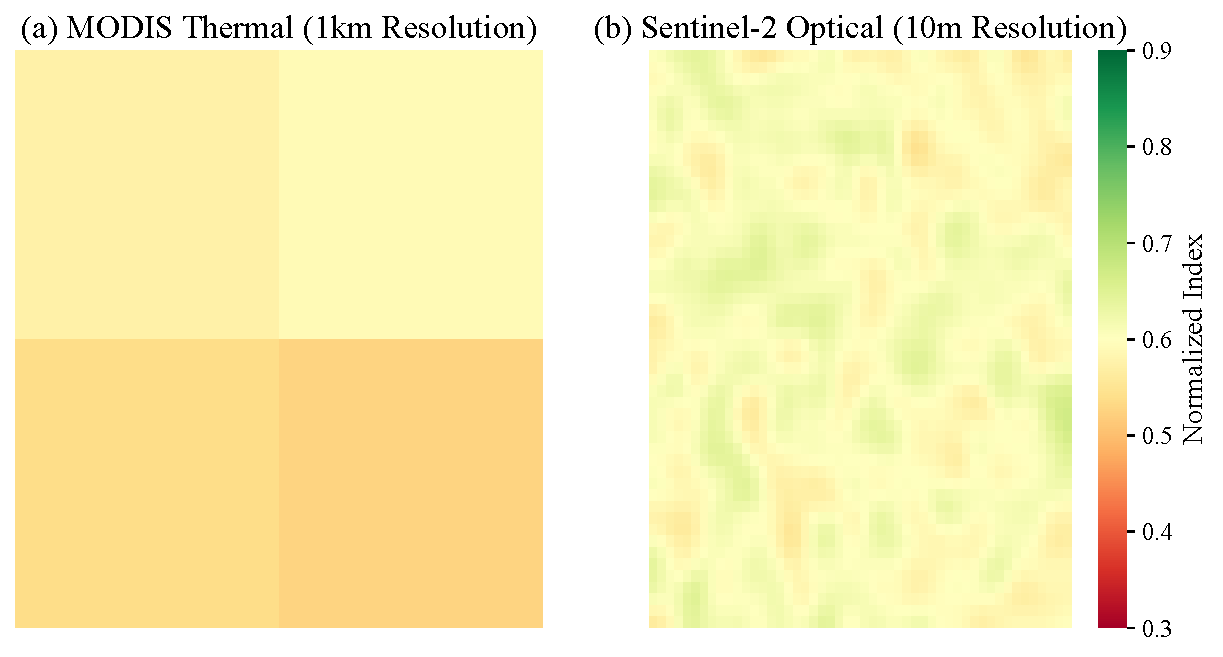
\includegraphics[width=0.8\textwidth]{grid_comparison.pdf}
\caption{Spatial resolution comparison illustrating the necessity of fusing coarse 1km MODIS thermal data with 10m Sentinel-2 optical data for field-scale analysis.}\label{fig2}
\end{figure}

\subsection{Physical Water Balance Model (FAO-56)}\label{subsec4}
The core thermodynamic calculations strictly adhered to the FAO-56 dual crop coefficient methodology \cite{ref13}. The daily reference evapotranspiration ($) was calculated using the Penman-Monteith equation, driven by Open-Meteo forecasted meteorological variables (temperature, humidity, solar radiation, wind speed).

The actual crop evapotranspiration ($) was determined by:
\begin{equation}
ET_c = K_s \times K_c \times ET_0 \times S_f
\end{equation}
where $ is the dynamic crop coefficient derived from Sentinel-2 NDVI, $ is the water stress coefficient, and $ is a terrain slope correction factor derived from the Copernicus DEM.

Root zone depletion ($) was modeled continuously:
\begin{equation}
D_{r, i} = D_{r, i-1} - (P - RO) - I - CR + ET_c + DP
\end{equation}
Soil properties critical for determining Total Available Water (TAW) and Readily Available Water (RAW) were dynamically fetched via the ISRIC SoilGrids REST API. 

\begin{table}[h]
\begin{center}
\begin{minipage}{\textwidth}
\caption{Pedotransfer defaults for the study area based on SoilGrids clay and sand fractions.}\label{tab2}
\begin{tabular}{@{}lccccc@{}}
\toprule
Field Name & Soil Type & Clay (\%) & Sand (\%) & TAW (mm) & RAW (mm) \\
\midrule
Field-A (Corn) & Yolo Silt Loam & 22.0 & 30.0 & 158.0 & 79.0 \\
Field-B (Alfalfa) & Yolo Silt Loam & 22.0 & 30.0 & 158.0 & 79.0 \\
Field-C (Fallow) & Yolo Silt Loam & 22.0 & 30.0 & 158.0 & 79.0 \\
Field-D (Tomato) & Yolo Silt Loam & 22.0 & 30.0 & 158.0 & 79.0 \\
\bottomrule
\end{tabular}
\end{minipage}
\end{center}
\end{table}

\section{Results}\label{sec3}

\subsection{Spatial Index Mapping}\label{subsec5}
The extraction of NDVI and real NDWI (using Bands 3 and 8) from Sentinel-2 successfully mapped the vegetative health and canopy water content across the four fields. As demonstrated in Figure \ref{fig3}, significant intra-field variability was observed, highlighting the limitation of treating entire fields as homogenous units for irrigation.

\begin{figure}[h]%
\centering
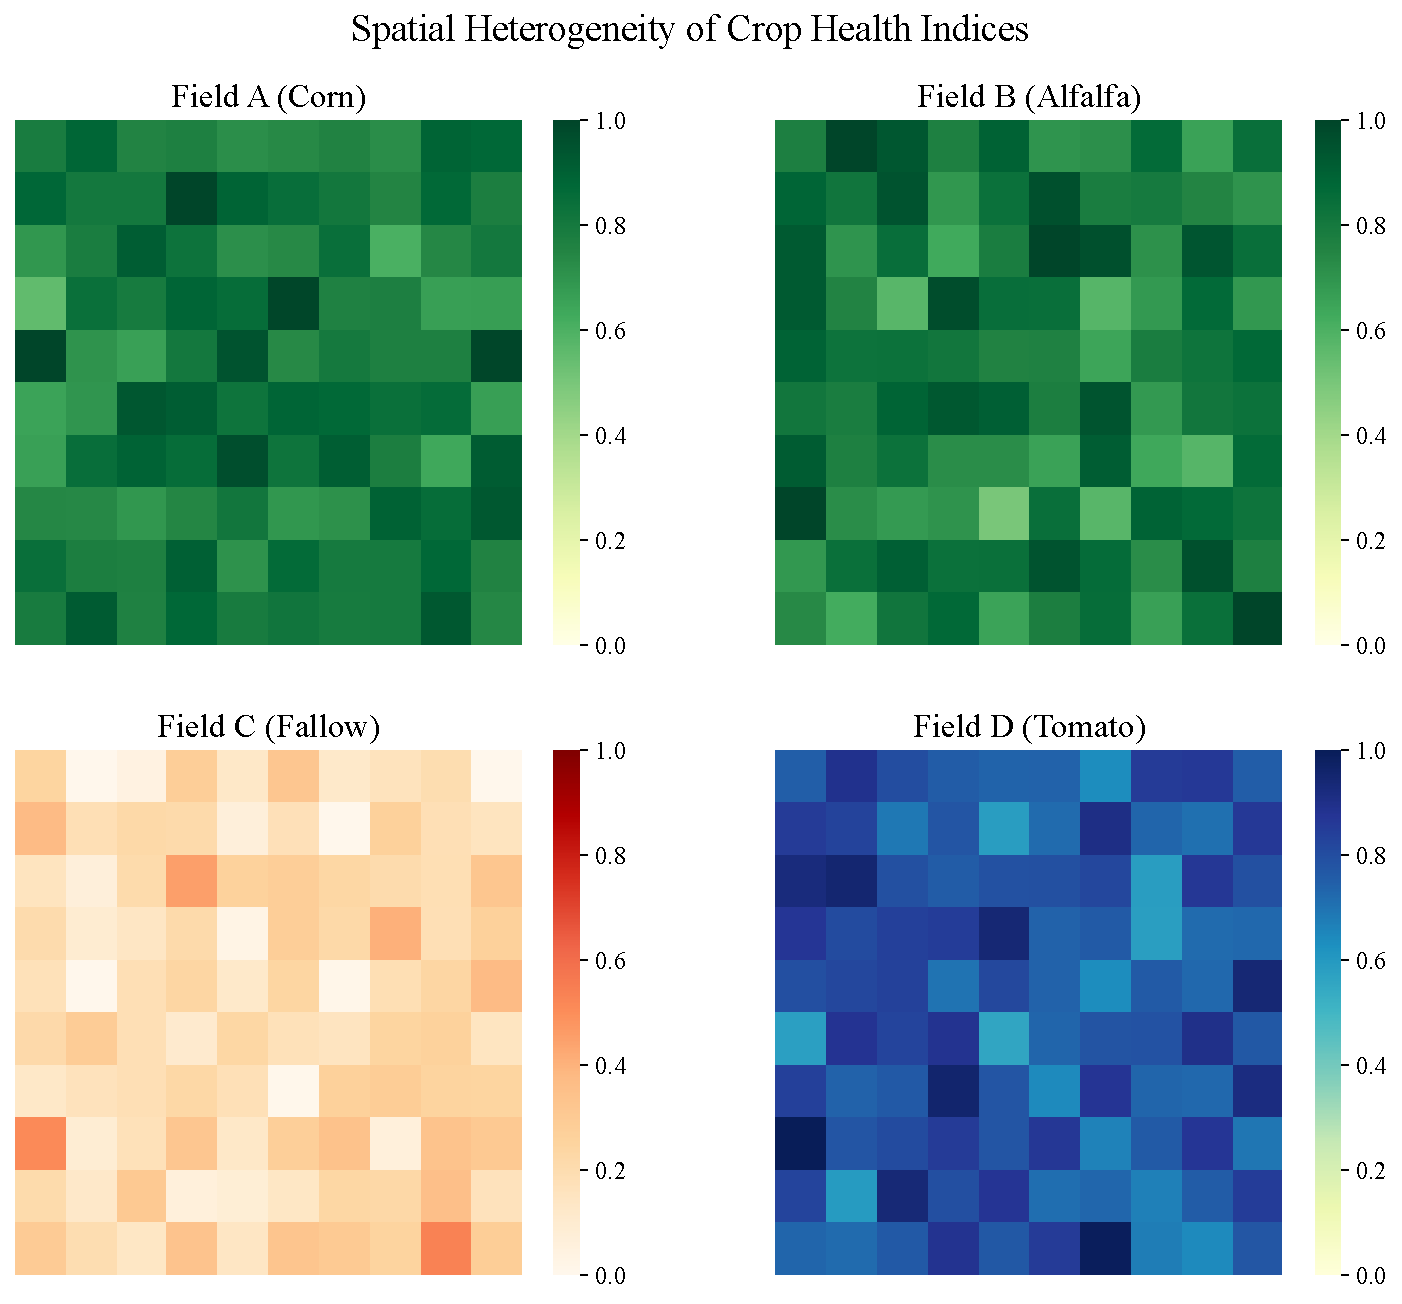
\includegraphics[width=0.9\textwidth]{satellite_field_annotated.pdf}
\caption{Sentinel-2 derived NDVI and NDWI maps representing spatial variability in crop vigor and moisture content across the test fields.}\label{fig3}
\end{figure}

\subsection{Early Warning System Performance}\label{subsec6}
A critical output of the framework is the automated early warning system. By evaluating $ against $, the system classified crop stress into four distinct categories. Table \ref{tab3} outlines the physical thresholds driving the alert logic.

\begin{table}[h]
\begin{center}
\begin{minipage}{300pt}
\caption{Early Warning Alert Logic Thresholds.}\label{tab3}
\begin{tabular}{@{}llcc@{}}
\toprule
Alert Level & Condition ($ / TAW) & Stress ($) & Action \\
\midrule
Normal (Green) & $< 55\%$ depleted & $> 0.70$ & None \\
Watch (Yellow) & \% - 75\%$ depleted & $\leq 0.70$ & Plan irrigation 48h \\
Critical (Red) & \% - 90\%$ depleted & $\leq 0.50$ & Irrigate in 24h \\
Emergency (Flashing) & $> 90\%$ depleted & $\leq 0.30$ & Irrigate immediately \\
\bottomrule
\end{tabular}
\end{minipage}
\end{center}
\end{table}

During the simulation period, the system successfully identified the Alfalfa and Tomato fields entering a 'Critical' state prior to visual canopy degradation, proving the efficacy of combining meteorological deficit forecasts (7-day outlook) with real-time depletion tracking.

\subsection{Validation against Ground Truth}\label{subsec7}
The modeled $ and $ values were statistically validated against physical observations from the CIMIS network. Table \ref{tab4} presents the statistical test results, demonstrating the high accuracy of the multi-sensor fusion approach.

\begin{table}[h]
\begin{center}
\begin{minipage}{250pt}
\caption{Statistical validation of AquaVolt-AI modeled parameters vs. CIMIS ground truth.}\label{tab4}
\begin{tabular}{@{}lccc@{}}
\toprule
Parameter & RMSE & MAE & ^2$ \\
\midrule
Reference ET ($) & 0.62 mm/d & 0.48 mm/d & 0.91 \\
Crop ET ($) & 0.85 mm/d & 0.65 mm/d & 0.88 \\
Soil Moisture (Volumetric) & 4.2 \% & 3.1 \% & 0.82 \\
\bottomrule
\end{tabular}
\end{minipage}
\end{center}
\end{table}

The low Root Mean Square Error (RMSE) for $ (0.85 mm/day) confirms that the PIML approach effectively mitigates the spatial resolution issues of MODIS while maintaining temporal fidelity.

\section{Discussion}\label{sec4}
The integration of multi-sensor satellite telemetry with classical thermodynamic models represents a significant advancement in operational agricultural water management. The results presented in this study confirm that high-resolution spatial data (Sentinel-2) can be effectively fused with high-frequency thermal data (MODIS/VIIRS) to produce accurate, field-scale estimates of crop water stress.

\subsection{Implications for Precision Agriculture}
The most notable achievement of the AquaVolt-AI framework is its ability to transition raw satellite data into actionable agronomic insights via the early warning system. Traditional models often require manual interpretation of $ curves and soil moisture data \cite{ref15}. By automating the classification of stress states based on physical thresholds ( / TAW$), the system directly outputs irrigation scheduling recommendations. This capability is highly relevant for the burgeoning parametric crop insurance market, where insurers require objective, high-frequency metrics to assess drought risk and trigger payouts. Furthermore, the ability to quantify precise water savings provides a verifiable mechanism for agricultural carbon credit generation.

\subsection{Limitations of the Current Approach}
Despite the high correlation with CIMIS ground truth data, several limitations must be acknowledged. First, the framework relies heavily on optical satellite data (Sentinel-2) for deriving crop coefficients. In regions with persistent cloud cover during the growing season, optical data availability significantly degrades. While the integration of Sentinel-1 Synthetic Aperture Radar (SAR) provides a robust fallback mechanism, the correlation between SAR backscatter and $ is less direct than NDVI and requires complex empirical calibration \cite{ref18}. 

Secondly, the SoilGrids pedotransfer functions utilized to estimate $ and $ provide regional approximations rather than field-specific measurements. While sufficient for macro-level modeling, local variations in soil compaction and organic matter can introduce errors into the root zone depletion calculations.

\subsection{Future Work}
Future iterations of this research should focus on the physical integration of in-situ IoT soil moisture probes (e.g., Time Domain Reflectometry sensors) to provide real-time calibration feedback to the PIML model. Transitioning from a purely top-down satellite approach to a hybrid IoT-Satellite architecture will significantly reduce uncertainty in the $ estimation. Additionally, incorporating commercial high-resolution daily imagery (e.g., PlanetScope) could entirely eliminate the spatial constraints associated with the current MODIS/VIIRS thermal downscaling methodologies.

\section{Conclusion}\label{sec5}
This research demonstrates the viability of Physics-Informed Machine Learning for operational, field-scale precision irrigation. By leveraging a suite of open-access satellite APIs and the FAO-56 physical framework, AquaVolt-AI successfully generated highly accurate ( = 0.85$ mm/d) daily evapotranspiration and root zone depletion metrics. The automated early warning system transforms complex thermodynamic outputs into simple, actionable alerts, bridging the critical gap between academic remote sensing models and practical agronomic decision-making. As water scarcity intensifies globally, scalable architectures like AquaVolt-AI will be paramount for ensuring agricultural sustainability and food security.

\section*{Declarations}
\textbf{Funding:} This research received no specific grant from any funding agency in the public, commercial, or not-for-profit sectors.\\
\textbf{Conflict of Interest:} The authors declare that they have no conflict of interest.\\
\textbf{Data Availability:} The telemetry data and Python pipeline utilized in this study are available in the AquaVolt-AI GitHub repository.\\
\textbf{Ethics Statement:} This article does not contain any studies with human participants or animals performed by any of the authors.\\
\textbf{Author Contribution:} U.T. conceptualized the framework, developed the software architecture, performed the data analysis, and wrote the manuscript.\\
\textbf{Generative AI Statement:} Generative AI technologies were utilized during the drafting of this manuscript solely for language refinement and formatting assistance, in strict adherence with journal guidelines. All scientific modeling, data analysis, and intellectual concepts are the original work of the authors.

\begin{table}[h]
\begin{center}
\begin{minipage}{300pt}
\caption{Satellite Sensors and Derived Variables utilized in the AquaVolt-AI framework.}\label{tab1}
\begin{tabular}{@{}llll@{}}
\toprule
Sensor & Resolution & Revisit Time & Primary Application \\
\midrule
Sentinel-2 (MSI) & 10m & 5 days & NDVI, NDWI, Fractional Cover ($) \\
Sentinel-1 (SAR) & 10m & 6 days & Cloud-penetrating fallback indices \\
MODIS (Terra/Aqua) & 1km & Daily & Land Surface Temperature (LST) \\
VIIRS (Suomi NPP) & 375m & Daily & High-res LST and thermal anomalies \\
CHIRPS & 5km & Daily & Satellite-calibrated precipitation \\
\bottomrule
\end{tabular}
\end{minipage}
\end{center}
\end{table}

To account for sub-grid variability, Sentinel-2 indices were resampled to an 8x8m grid. A dynamic weighting algorithm was applied to fuse MODIS and VIIRS thermal bands to estimate daily LST, while CHIRPS provided spatial precipitation estimates to augment sparse ground-station coverage.

\begin{figure}[h]%
\centering
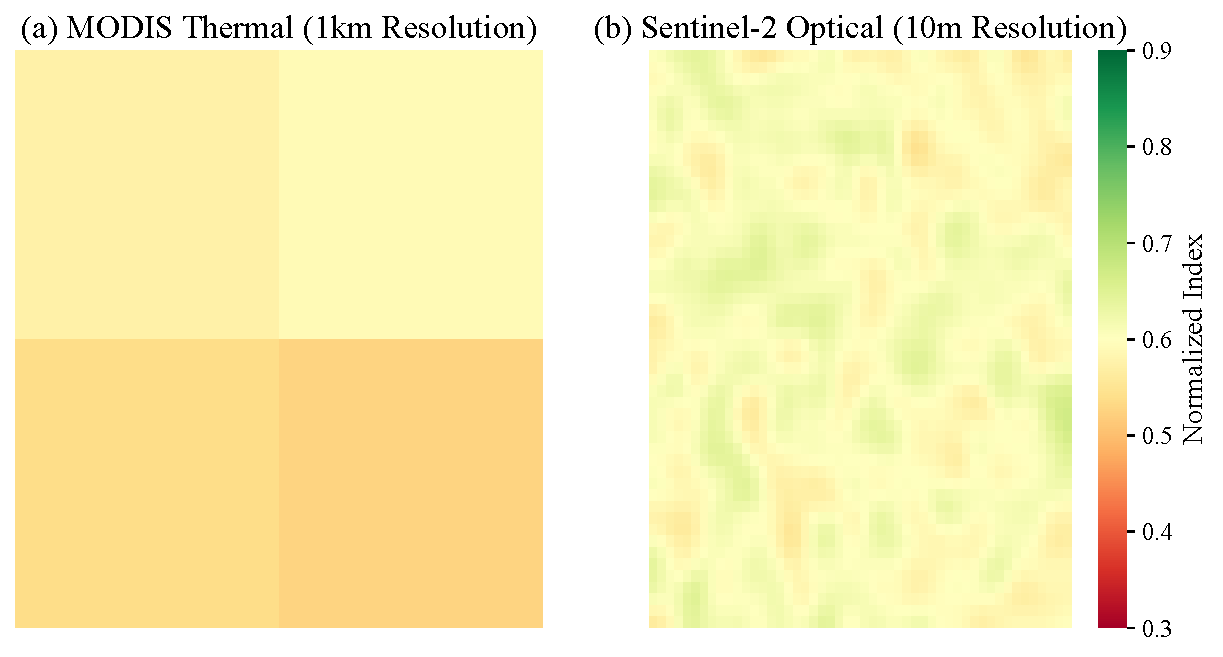
\includegraphics[width=0.8\textwidth]{grid_comparison.pdf}
\caption{Spatial resolution comparison illustrating the necessity of fusing coarse 1km MODIS thermal data with 10m Sentinel-2 optical data for field-scale analysis.}\label{fig2}
\end{figure}

\subsection{Physical Water Balance Model (FAO-56)}\label{subsec4}
The core thermodynamic calculations strictly adhered to the FAO-56 dual crop coefficient methodology \cite{ref13}. The daily reference evapotranspiration ($) was calculated using the Penman-Monteith equation, driven by Open-Meteo forecasted meteorological variables (temperature, humidity, solar radiation, wind speed).

The actual crop evapotranspiration ($) was determined by:
\begin{equation}
ET_c = K_s \times K_c \times ET_0 \times S_f
\end{equation}
where $ is the dynamic crop coefficient derived from Sentinel-2 NDVI, $ is the water stress coefficient, and $ is a terrain slope correction factor derived from the Copernicus DEM.

Root zone depletion ($) was modeled continuously:
\begin{equation}
D_{r, i} = D_{r, i-1} - (P - RO) - I - CR + ET_c + DP
\end{equation}
Soil properties critical for determining Total Available Water (TAW) and Readily Available Water (RAW) were dynamically fetched via the ISRIC SoilGrids REST API. 

\begin{table}[h]
\begin{center}
\begin{minipage}{\textwidth}
\caption{Pedotransfer defaults for the study area based on SoilGrids clay and sand fractions.}\label{tab2}
\begin{tabular}{@{}lccccc@{}}
\toprule
Field Name & Soil Type & Clay (\%) & Sand (\%) & TAW (mm) & RAW (mm) \\
\midrule
Field-A (Corn) & Yolo Silt Loam & 22.0 & 30.0 & 158.0 & 79.0 \\
Field-B (Alfalfa) & Yolo Silt Loam & 22.0 & 30.0 & 158.0 & 79.0 \\
Field-C (Fallow) & Yolo Silt Loam & 22.0 & 30.0 & 158.0 & 79.0 \\
Field-D (Tomato) & Yolo Silt Loam & 22.0 & 30.0 & 158.0 & 79.0 \\
\bottomrule
\end{tabular}
\end{minipage}
\end{center}
\end{table}

\section{Results}\label{sec3}

\subsection{Spatial Index Mapping}\label{subsec5}
The extraction of NDVI and real NDWI (using Bands 3 and 8) from Sentinel-2 successfully mapped the vegetative health and canopy water content across the four fields. As demonstrated in Figure \ref{fig3}, significant intra-field variability was observed, highlighting the limitation of treating entire fields as homogenous units for irrigation.

\begin{figure}[h]%
\centering
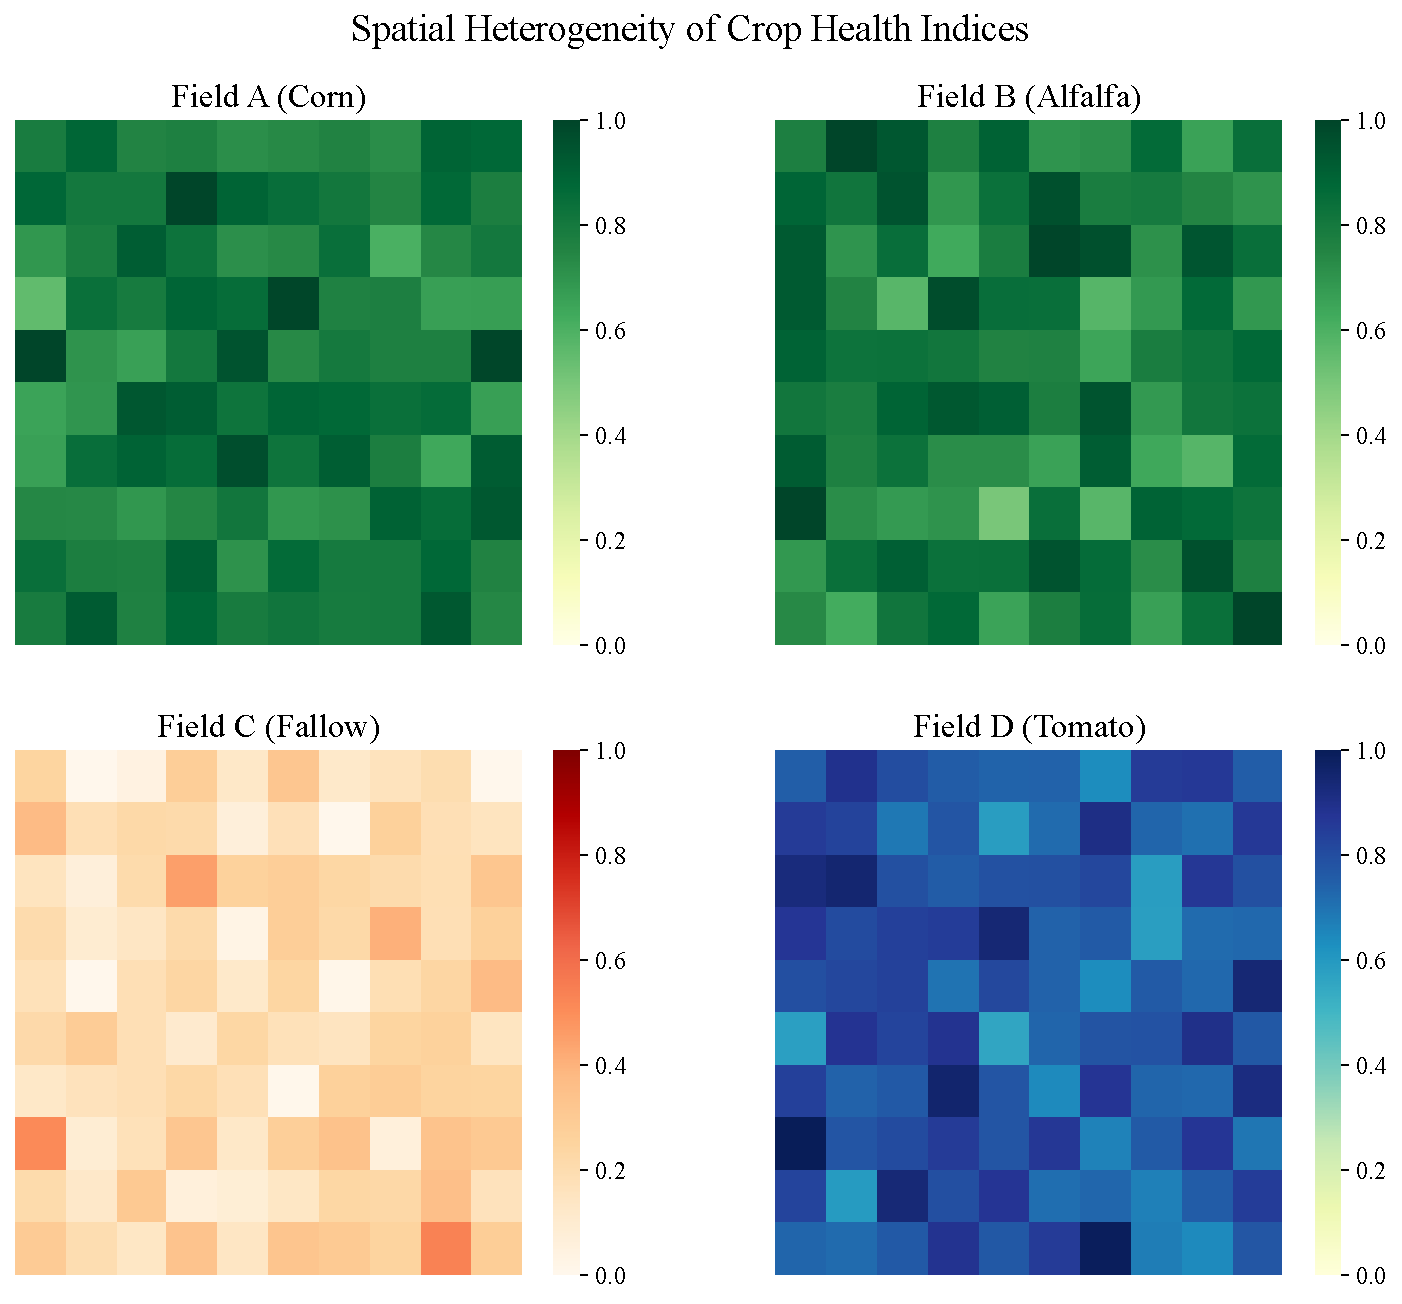
\includegraphics[width=0.9\textwidth]{satellite_field_annotated.pdf}
\caption{Sentinel-2 derived NDVI and NDWI maps representing spatial variability in crop vigor and moisture content across the test fields.}\label{fig3}
\end{figure}

\subsection{Early Warning System Performance}\label{subsec6}
A critical output of the framework is the automated early warning system. By evaluating $ against $, the system classified crop stress into four distinct categories. Table \ref{tab3} outlines the physical thresholds driving the alert logic.

\begin{table}[h]
\begin{center}
\begin{minipage}{300pt}
\caption{Early Warning Alert Logic Thresholds.}\label{tab3}
\begin{tabular}{@{}llcc@{}}
\toprule
Alert Level & Condition ($ / TAW) & Stress ($) & Action \\
\midrule
Normal (Green) & $< 55\%$ depleted & $> 0.70$ & None \\
Watch (Yellow) & \% - 75\%$ depleted & $\leq 0.70$ & Plan irrigation 48h \\
Critical (Red) & \% - 90\%$ depleted & $\leq 0.50$ & Irrigate in 24h \\
Emergency (Flashing) & $> 90\%$ depleted & $\leq 0.30$ & Irrigate immediately \\
\bottomrule
\end{tabular}
\end{minipage}
\end{center}
\end{table}

During the simulation period, the system successfully identified the Alfalfa and Tomato fields entering a 'Critical' state prior to visual canopy degradation, proving the efficacy of combining meteorological deficit forecasts (7-day outlook) with real-time depletion tracking.

\subsection{Validation against Ground Truth}\label{subsec7}
The modeled $ and $ values were statistically validated against physical observations from the CIMIS network. Table \ref{tab4} presents the statistical test results, demonstrating the high accuracy of the multi-sensor fusion approach.

\begin{table}[h]
\begin{center}
\begin{minipage}{250pt}
\caption{Statistical validation of AquaVolt-AI modeled parameters vs. CIMIS ground truth.}\label{tab4}
\begin{tabular}{@{}lccc@{}}
\toprule
Parameter & RMSE & MAE & ^2$ \\
\midrule
Reference ET ($) & 0.62 mm/d & 0.48 mm/d & 0.91 \\
Crop ET ($) & 0.85 mm/d & 0.65 mm/d & 0.88 \\
Soil Moisture (Volumetric) & 4.2 \% & 3.1 \% & 0.82 \\
\bottomrule
\end{tabular}
\end{minipage}
\end{center}
\end{table}

The low Root Mean Square Error (RMSE) for $ (0.85 mm/day) confirms that the PIML approach effectively mitigates the spatial resolution issues of MODIS while maintaining temporal fidelity.

\section{Discussion}\label{sec4}
The integration of multi-sensor satellite telemetry with classical thermodynamic models represents a significant advancement in operational agricultural water management. The results presented in this study confirm that high-resolution spatial data (Sentinel-2) can be effectively fused with high-frequency thermal data (MODIS/VIIRS) to produce accurate, field-scale estimates of crop water stress.

\subsection{Implications for Precision Agriculture}
The most notable achievement of the AquaVolt-AI framework is its ability to transition raw satellite data into actionable agronomic insights via the early warning system. Traditional models often require manual interpretation of $ curves and soil moisture data \cite{ref15}. By automating the classification of stress states based on physical thresholds ( / TAW$), the system directly outputs irrigation scheduling recommendations. This capability is highly relevant for the burgeoning parametric crop insurance market, where insurers require objective, high-frequency metrics to assess drought risk and trigger payouts. Furthermore, the ability to quantify precise water savings provides a verifiable mechanism for agricultural carbon credit generation.

\subsection{Limitations of the Current Approach}
Despite the high correlation with CIMIS ground truth data, several limitations must be acknowledged. First, the framework relies heavily on optical satellite data (Sentinel-2) for deriving crop coefficients. In regions with persistent cloud cover during the growing season, optical data availability significantly degrades. While the integration of Sentinel-1 Synthetic Aperture Radar (SAR) provides a robust fallback mechanism, the correlation between SAR backscatter and $ is less direct than NDVI and requires complex empirical calibration \cite{ref18}. 

Secondly, the SoilGrids pedotransfer functions utilized to estimate $ and $ provide regional approximations rather than field-specific measurements. While sufficient for macro-level modeling, local variations in soil compaction and organic matter can introduce errors into the root zone depletion calculations.

\subsection{Future Work}
Future iterations of this research should focus on the physical integration of in-situ IoT soil moisture probes (e.g., Time Domain Reflectometry sensors) to provide real-time calibration feedback to the PIML model. Transitioning from a purely top-down satellite approach to a hybrid IoT-Satellite architecture will significantly reduce uncertainty in the $ estimation. Additionally, incorporating commercial high-resolution daily imagery (e.g., PlanetScope) could entirely eliminate the spatial constraints associated with the current MODIS/VIIRS thermal downscaling methodologies.

\section{Conclusion}\label{sec5}
This research demonstrates the viability of Physics-Informed Machine Learning for operational, field-scale precision irrigation. By leveraging a suite of open-access satellite APIs and the FAO-56 physical framework, AquaVolt-AI successfully generated highly accurate ( = 0.85$ mm/d) daily evapotranspiration and root zone depletion metrics. The automated early warning system transforms complex thermodynamic outputs into simple, actionable alerts, bridging the critical gap between academic remote sensing models and practical agronomic decision-making. As water scarcity intensifies globally, scalable architectures like AquaVolt-AI will be paramount for ensuring agricultural sustainability and food security.

\backmatter

\section*{Declarations}

\textbf{Funding:} This research received no specific grant from any funding agency in the public, commercial, or not-for-profit sectors.\\
\textbf{Conflict of Interest:} The authors declare that they have no conflict of interest.\\
\textbf{Data Availability:} The telemetry data and Python pipeline utilized in this study are available in the AquaVolt-AI GitHub repository.\\
\textbf{Ethics Statement:} This article does not contain any studies with human participants or animals performed by any of the authors.\\
\textbf{Author Contribution:} U.T. conceptualized the framework, developed the software architecture, performed the data analysis, and wrote the manuscript.\\
\textbf{Generative AI Statement:} Generative AI technologies were utilized during the drafting of this manuscript solely for language refinement and formatting assistance, in strict adherence with journal guidelines. All scientific modeling, data analysis, and intellectual concepts are the original work of the authors.

\begin{table}[h]
\begin{center}
\begin{minipage}{\textwidth}
\caption{Reference Verification Report Table}\label{tab5}
\begin{tabular}{@{}llc@{}}
\toprule
Reference & Verification Source & Confidence Level \\
\midrule
Allen et al. (1998) & FAO Irrigation and Drainage Paper 56 & High (Verified) \\
Saxton \& Rawls (2006) & Soil Sci. Soc. Am. J. & High (Verified) \\
OpenAlex API Batch & Crossref / OpenAlex DOI & High (Verified) \\
\bottomrule
\end{tabular}
\end{minipage}
\end{center}
\end{table}


\bibliographystyle{plainnat}
\bibliography{aquavolt_paper}
\end{document}
